
%(BEGIN_QUESTION)
% Copyright 2011, Tony R. Kuphaldt, released under the Creative Commons Attribution License (v 1.0)
% This means you may do almost anything with this work of mine, so long as you give me proper credit

Dette temperaturreguleringssystemet for en ovn fungerer ikke godt nok. Temperaturen driver rundt settpunktet, til tross for flere forsøk på tuning av P-, I- og D-parametere.

$$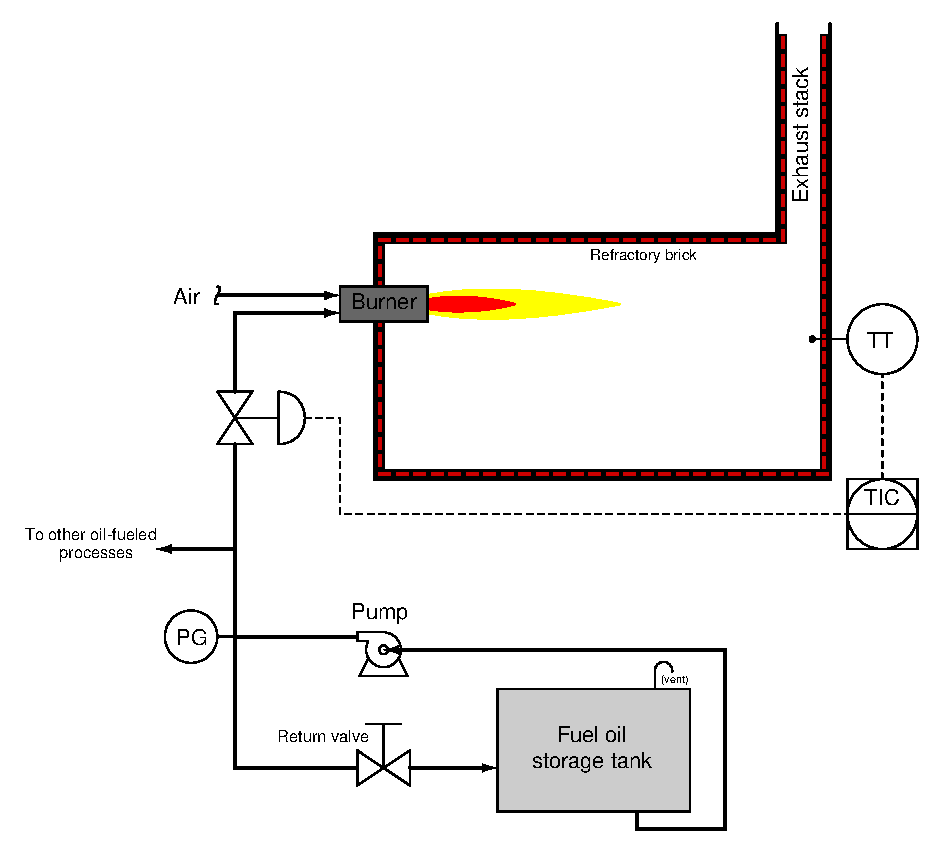
\includegraphics[width=15.5cm]{i00714x01.eps}$$

En instrumenttekniker ser til slutt at trykkindikeringen på utløpet av oljepumpen er ustabil og varierer tilsynelatende tilfeldig.

\vskip 10pt

Vis hvordan temperaturstabiliteten kan forbedres ved å innføre kaskaderegulering.

\vskip 20pt \vbox{\hrule \hbox{\strut \vrule{} {\bf Forslag til sokratisk diskusjon} \vrule} \hrule}

\begin{itemize}
\item{} Finnes det andre løsninger enn kaskade for dette problemet?
\item{} Hvorfor tror du det finnes en returventil i fyringsoljekretsen?
\item{} Forklar hva som skjer hvis noen plutselig stenger returventilen fra normal posisjon.
\item{} Forklar hva som skjer hvis noen plutselig åpner returventilen mer enn normalt.
\end{itemize}

\underbar{file i00714no}
%(END_QUESTION)





%(BEGIN_ANSWER)

Det finnes flere løsninger på problemet. Her er én:

$$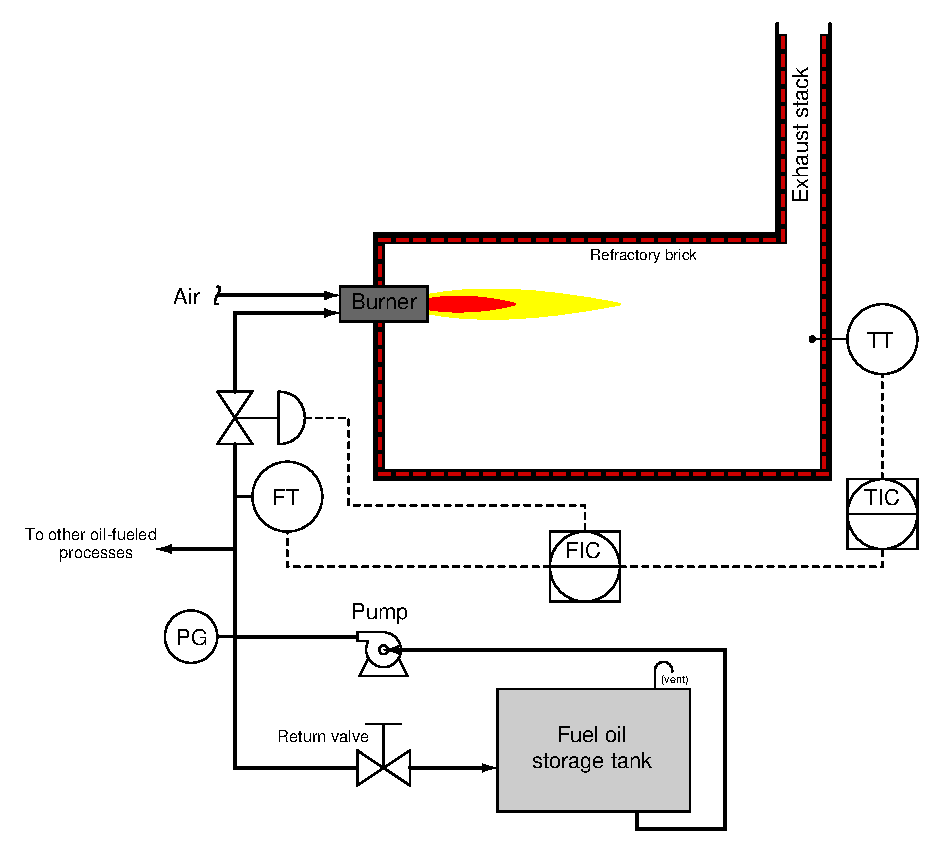
\includegraphics[width=15.5cm]{i00714x02.eps}$$

%(END_ANSWER)





%(BEGIN_NOTES)

Her er en løsning som ikke baserer seg på kaskade eller annen strategi i seg selv:

$$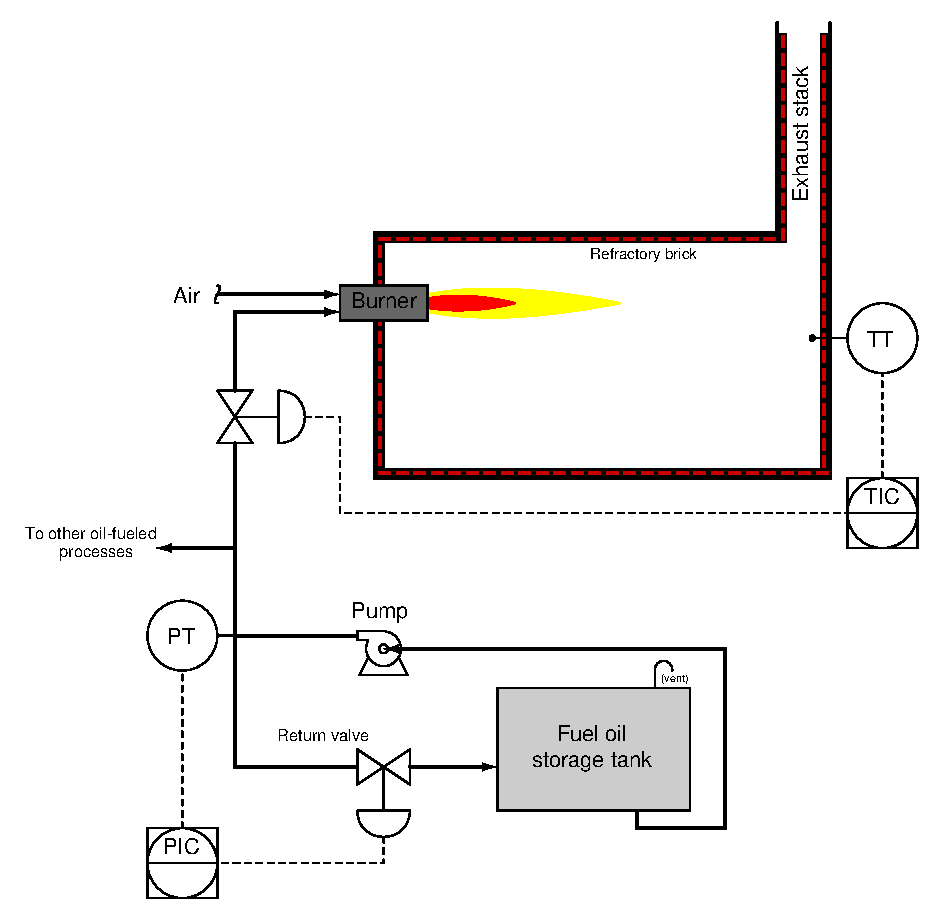
\includegraphics[width=15.5cm]{i00714x03.eps}$$

%INDEX% Regulering, strategier: kaskade
%INDEX% Prosess: forbrenningsovn

%(END_NOTES)
